\documentclass[a4paper]{article}

%image insertion
\usepackage{graphicx} %image settings
\DeclareGraphicsExtensions{.pdf,.png,.jpg}

%math
\usepackage{amsmath} %math
%\usepackage{cmbright} %math font

%font
\usepackage{kotex}
\usepackage{fontspec}
\ifx가가
\setmainhangulfont[Ligatures=TeX,
BoldFont={KoPubBatang Medium}]{KoPubBatang Light}
\setsanshangulfont[Ligatures=TeX,
BoldFont={KoPubDotum Medium}]{KoPubDotum Light}
\setmainhanjafont[Ligatures=TeX,
BoldFont={KoPubBatang Medium}]{KoPubBatang Light}
\setsanshanjafont[Ligatures=TeX,
BoldFont={KoPubDotum Medium}]{KoPubDotum Light}
\xetexkofontregime[puncts=prevfont, colons=prevfont, cjksymbols=hangul]{latin}
\fi

%줄간격
\usepackage{setspace}
\usepackage{indentfirst}
\setstretch{1.3}
\everydisplay{\setstretch{1.2}}

%subfigure
\usepackage{subfigure}

\pagestyle{plain}
\title{물리 실험보고서 1}
\author{이한빈, 의예과 2016-13347}

\begin{document}


\numberwithin{equation}{section}
\maketitle

\section{Introduction}
	폐회로가 주어졌을 때 회로 내부를 지나가는 자기선속이 변하면 크기는 시간당 변화량에 비례하며 방향은 자기선속 변화의 반대인 기전력이 회로에 유도된다.
	이를 페러데이의 법칙이라고 하며 다음과 같이 표현된다.
	\begin{equation}
		\epsilon = -\frac{d\Phi}{dt}
	\end{equation}
	여기서 기전력의 방향이 자기선속 변화의 반대라는 사실을 렌츠의 법칙이라고 부른다.

	페러데이의 법칙을 이용하면 전동기에서 발생하는 기전력을 계산할 수 있다.
	회로의 면적을 $A$, 회전각속력을 $\omega$, 회로가 놓여진 공간의 자기장을 $B$라고 하자.
	\begin{figure}[h]
		\centering
		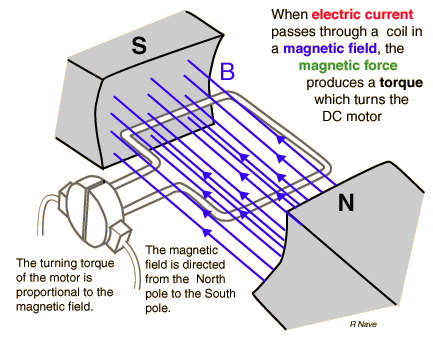
\includegraphics[width=0.6\textwidth]{img/motor.png}
	\end{figure}






\section{Reference}
	1. Halliday, D., Resnick, R., \& Walker, J. (2014). {\it{}Principles of Physics} (10th ed., Vol. 2). Hoboken, NJ: Wiley. 

\end{document} 

%실험에서 개선할 점 등 피피티에서 봤던 거 모두 적어서 처리합시다